% Introduction to probability theory
    % - [x] Basic concepts such as events, outcomes, and sample spaces
    % - [x] Definition of probability and probability axioms
    % - [x] Definition of conditional probability
    % - [x] Bayes' rule and its derivation
    % - [x] Discrete and continuous probability distributions
    % - [x] Expectation, variance, and covariance
    % - [x] Known probability distributions and their properties

\renewcommand{\Pr}[1]{\operatorname{Pr}\{#1\}}

When we are dealing with probability of an event, we assume that there is a possibility
of that event occurring and we measure it using a number between 0 and 1 or a percentage
between 0\% and 100\%. In other words, we use the probability theory framework to assign
numerical values to arbitrary events. This section covers several fundamental concepts of
probability theory, which serve as the basis for this work.

The \textit{event}, which we formally denote as $E$, comes from some space of all possible
events, the \textit{outcome space} $\Omega$. We also denote the \textit{probability} of the
event $E$ as $\Pr{E}$. This probability is a real non-negative number,
that is $\Pr{E} \in \mathbb{R}, \Pr{E} \geq 0$. The outcome
space covers all possible events, that is $\Pr{\Omega} = 1$. It then follows
that the probability of disjoint events from the outcome space $\Omega$ is the sum of
probabilities of these events, that is for
$E_1, \ldots, E_n \in \Omega, \Pr{\bigcup_{i=1}^n E_i} = \sum_{i=1}^n \Pr{E_i}$.

We have defined three main axioms of probability theory. In addition to these axioms, several
crucial concepts illustrate the relationship between events. Given two events, $E_1$ and $E_2$,
the \textit{conditional probability} of $E_1$ given $E_2$ is defined as

$$
\Pr{E_1 \mid E_2} = \frac{\Pr{E_1 \cap E_2}}{\Pr{E_2}}.
$$

If the events are \textit{independent} of each other, the probability of them occurring
simultaneously is given by

$$
\Pr{E_1 \cap E_2} = \Pr{E_1}\Pr{E_2}.
$$

These relationships allow us to define the \textit{law of total probability}
\cite[31]{zwillingerCRCStandardProbability2000}, which is a key component of Bayes' rule.
Let $A$ be an event, $A \int \Omega$, and $\{B_n : n = 1, 2, \ldots\}$ be a countable
partition of the space $\Omega$. Then, we have:

$$
\Pr{A} = \sum_n \Pr{A \mid B_n} \Pr{B_n}.
$$

Now, we can deduce the following rule:

\begin{definition}[Bayes' rule]
Let $A$ and $B$ be two events from the outcome space $\Omega$. Then the following applies:

$$
\Pr{A \mid B} = \frac{\Pr{B \mid A}}{\Pr{B}}
    = \frac{\Pr{B \mid A}}{\sum_n \Pr{B \mid A_n}\Pr{A_n}}.
$$
\end{definition}

Bayes' rule plays a crucial role in Bayesian inference and serves as the basis for
Bayesian filters, including the PHD filter.

\subsection{Probability distributions}

Events and their probabilities are not sufficient for our purposes;
we need a framework that allows us to obtain a formal, general description of a set
of events from some outcome space. Specifically, we need an abstraction around events,
which is some function that maps the outcome space $\Omega$ to some other space,
typically $\mathbb{R}$ (but not necessarily). This abstraction is called a
\textit{random variable} and one outcome of it is called a \textit{realization}.

\begin{definition}[Random variable and its realization]
    Let $\Omega$ be a set of possible events, $\omega \in \Omega$ is some event,
    and $\mathbb{O}$ be another space. A function $X: \Omega \rightarrow \mathbb{O}$
    is called a random variable and $x = X(\omega)$ is called a realization of $X$.
\end{definition}

The above definition provides a general framework for understanding random variables.
However, for the purposes of Bayesian statistics, we will simplify the discussion by
focusing on scalar, continuous-valued random variables, represented
by $\mathbb{O} = \mathbb{R}$. In practice, it is often impractical to calculate the
probability of every possible event from the outcome space $\Omega$, especially for
continuous random variables with uncountably infinite outcomes. Instead, it may suffice
to work with intervals on the outcome space and their probabilities. We call such a
probability distribution a \textit{cumulative distribution function (cdf)} of $X$,
and the first-order derivative of the cdf is called a \textit{probability density
function (pdf)}.\footnote{
    For discrete random variables, the corresponding distribution function is
    called a \textit{probability mass function (pmf)}.
}

\begin{definition}[Cumulative distribution function (cdf)]
    Given a scalar real-valued random variable $X \in \mathbb{R}$ and $x$ as a
    realization of $X$, we define the probability $\Pr{X \in (-\infty, x)} = \Pr{X < x}$
    as the cumulative distribution function of random variable $X$ and denote it as $P(x)$.
\end{definition}

\begin{definition}[Probability density function (pdf)]
    The probability density function $p(x)$ of a scalar real-valued random variable $X$
    is defined as:
    $$
    p(x) = \frac{\partial P(x)}{\partial x}.
    $$
\end{definition}

Probability distributions are fundamental in Bayesian statistics and provide a way
to model and analyze the behavior of random variables. In the next section,
we will discuss some common probability distributions used in Bayesian filters,
including the Gaussian distribution and the Poisson distribution.

Probability distributions are fundamental in Bayesian statistics and provide a way
to model and analyze the behavior of random variables. Cdfs and pdfs (as well as pmfs
for discrete cases) are used to specify the probability distribution of a random
variable, providing a formal description of the relationship
between events and probabilities. In addition to this formal description, we also
need to know several statistical properties of probability distributions to fully
understand their behavior. Two main properties of probability distributions are
the expected value, $E[X]$, and the variance, $\operatorname{Var}[X]$:

$$
\begin{aligned}
E[X]&=\int_{-\infty}^{\infty} x p(x) d x \\
\operatorname{Var}[X]
    &= E\left[(X-E[X])^2\right]
    =\int_{-\infty}^{\infty}(x-E[X])^2 p(x) d x.
\end{aligned}
$$

The expected value, or the first moment, represents the most probable value of
a random variable. The variance, or the second central moment, is a measure of the
variability of a random variable and is often denoted as $\operatorname{Var}[X] = \sigma^2$.
Furthermore, we often study the relationship between two random variables, say $X$ and
$Y$, and measure their joint variability, which we call a \textit{covariance}:

$$
\operatorname{Cov}[X, Y]
    = E\left[(X-E[X])(Y-E[Y])\right]
    =\int_{-\infty}^{\infty}(x-E[X])(y-E[Y]) p(x, y) d x d x.
$$

For vector-valued random variables, that is $X, Y \in \mathbb{R}^k$ and $\mathbf{x}$
is the realization of $X$, the formulas are the following. It is worth noting that
the covariance in the vector case becomes a matrix and is called a \textit{covariance
matrix}:

$$
\begin{aligned}
E[X]
    &=\int_{-\infty}^{\infty} \mathbf{x} p(\mathbf{x}) d \mathbf{x} \\
\operatorname{Var}(X)
    &= E\left[\left(X-E[X]\right)\left(X-E[X]\right)^\intercal\right]
    \\&=\int_{-\infty}^{\infty}
        \left(\mathbf{x}-E[X]\right)
        \left(\mathbf{x}-E[X]\right)^\intercal
        p(\mathbf{x})
        d \mathbf{x} \\
\operatorname{Cov}[X, Y]
    &= E\left[\left(X-E[X]\right)\left(Y-E[Y]\right)^\intercal\right]
    \\&=\int_{-\infty}^{\infty}
        \left(\mathbf{x}-E[X]\right)
        \left(\mathbf{y}-E[Y]\right)^\intercal
        p(\mathbf{x}, \mathbf{y})
        d \mathbf{x} d \mathbf{y}.
\end{aligned}
$$

Probability distributions are fundamental in Bayesian statistics and
provide a way to model and analyze the behavior of random variables. For
the purpose of Bayesian filters, some common probability distributions
are particularly useful. In this section, we will discuss some of these
distributions and their main properties. We shall start from discrete
cases and go on to the continuous variables.  % uniform, bernoulli, poisson, gaussian

\subsubsection{Bernoulli distribution}

The Bernoulli distribution is the simplest discrete probability
distribution, and the Bernoulli random variable is binary, with only
two realizations, $0$ or $1$. This distribution is parameterized with 
$r$, the probability of the positive outcome. Its probability mass 
function is given by

$$
p(x) = \begin{cases}
 1 - r, & \text{if } x = 0, \\
     r, & \text{if } x = 1, \\
     0, & \text{otherwise}.
\end{cases}
$$

\begin{figure}
\centering
\begin{subfigure}{.5\textwidth}
  \centering
  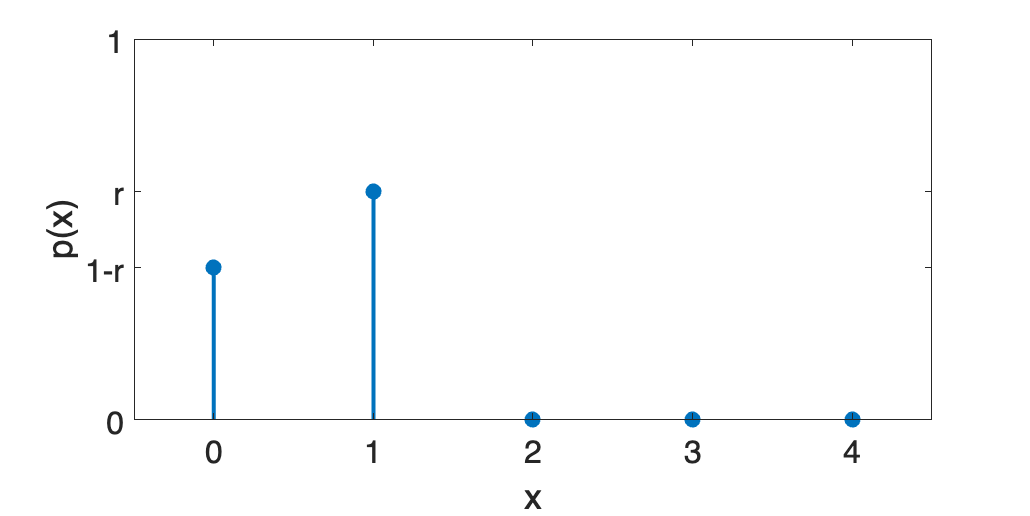
\includegraphics[width=.9\linewidth]{figures/bern.pmf.png}
  \caption{PMF.}
  \label{fig:bern:pmf}
\end{subfigure}%
\begin{subfigure}{.5\textwidth}
  \centering
  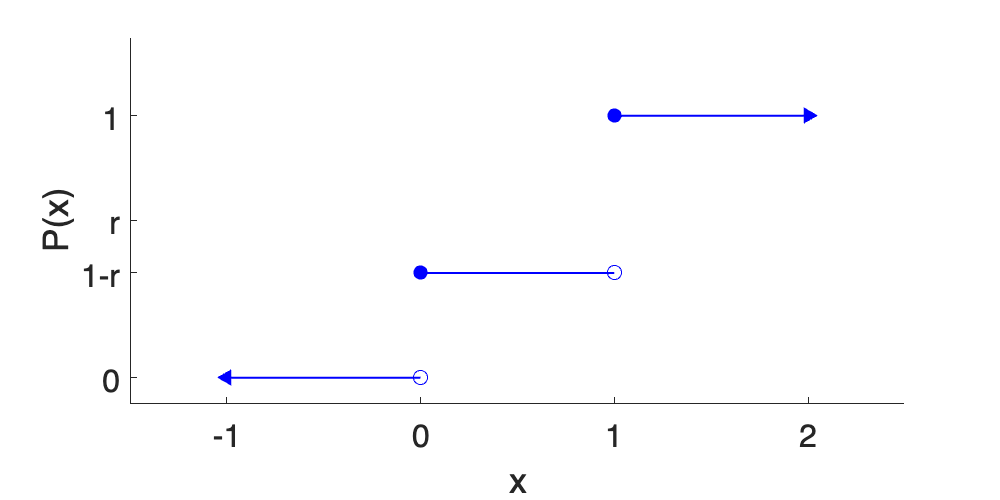
\includegraphics[width=.9\linewidth]{figures/bern.cdf.png}
  \caption{CDF.}
  \label{fig:bern:cdf}
\end{subfigure}
\caption{Bernoulli distribution.}
\label{fig:bern}
\end{figure}

The pmf and the cdf of the Bernoulli distribution can be seen on Figure \ref{fig:bern}.
We denote this distribution as $p(x) = \operatorname{Bernoulli}(x;r)$.
The expected value and the covariance of a Bernoulli random variable $X$ are

$$
E[X] = r, \qquad \operatorname{Var}[X] = r(1-r).
$$

In object tracking, we use Bernoulli random variables to model the existence of
an object at some time step $k$, which we will discuss in detail in the following
sections.

\subsubsection{Binomial distribution}

Binomial random variables are the generalization of Bernoulli random variables,
representing the probability of $x$ positive outcomes after $n$ consecutive and
independent trials. This distribution is parameterized by the probability of the
positive outcome in one trial $r$ and the number of trials $n$. Its pmf, as well 
as the expected value and the variance, are given by

$$
\begin{aligned}
    p(x) &= \binom{n}{x} r^x (1-r)^{(n-x)}, \\
    E[X] &= nr, \\
    \operatorname{Var}[X] &= nr(1-r).
\end{aligned}
$$

\subsubsection{Poisson distribution}

The Poisson distribution is a discrete random distribution that can 
be used as an approximation of the Binomial distribution in cases where 
$n$ tends towards infinity and $r$ tends towards $0$ such that their 
product stays about equal to a parameter $\lambda$, which is the 
parameter of the Poisson distribution and also its expected value and 
variance. The outcome space of a Poisson random variable is 
$\mathbb{N}_0$,\footnote{Natural numbers including $0$.} and its pmf,
expected value and variance are given by

$$
\begin{aligned}
    p(x) = \operatorname{Poisson}(x; \lambda) &= \frac{\lambda^x e^{-\lambda}}{x !}, \\
    E[X] = \operatorname{Var}[X] &= \lambda.
\end{aligned}
$$

The probability mass function and the corresponding cumulative density functions
of the Poisson distribution can be seen in Figure \ref{fig:poisson}.
The Poisson distribution is a critical component of modern multi-object
tracking systems, as it is used to model noise measurements, and some 
systems even use it to model objects that exist but are not visible in
the field of view of a sensor \cite{garcia-fernandezPoissonMultiBernoulliMixture2018}.
The Poisson distribution is the foundation of the so-called Poisson Point
Processes (PPP), which will be discussed later.

\begin{figure}
\centering
\begin{subfigure}{.5\textwidth}
  \centering
  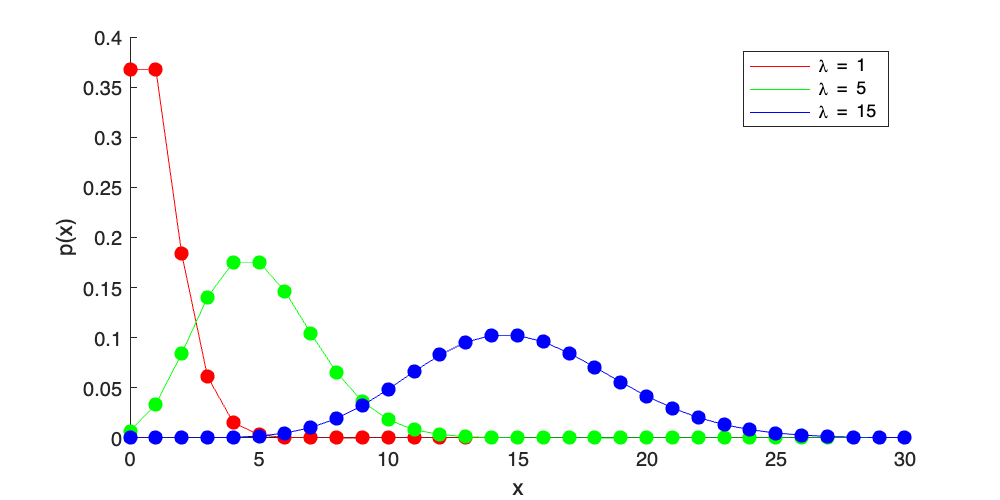
\includegraphics[width=.9\linewidth]{figures/poisson.pmf.png}
  \caption{PMF.}
  \label{fig:poisson:pmf}
\end{subfigure}%
\begin{subfigure}{.5\textwidth}
  \centering
  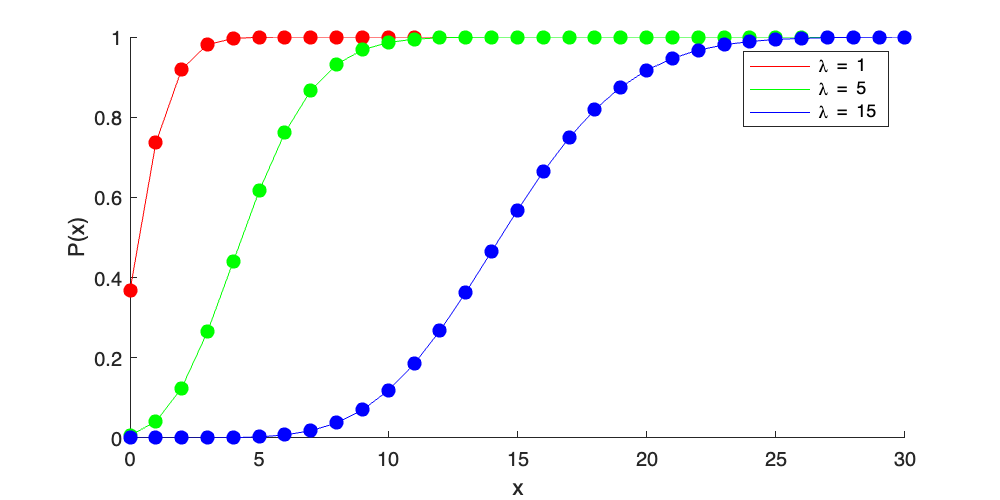
\includegraphics[width=.9\linewidth]{figures/poisson.cdf.png}
  \caption{CDF.}
  \label{fig:poisson:cdf}
\end{subfigure}
\caption{Poisson distribution.}
\label{fig:poisson}
\end{figure}

\subsubsection{Uniform distribution}

The uniform distribution is a continuous probability distribution and it
describes such random variables which outcomes on some interval $[a, b]$
are possible with equal probability. This distribution is parameterized by
$a$ and $b$ and its pdf, $E[X]$ and $\operatorname{Var}[X]$ are:

$$
\begin{aligned}
    p(x)
        =\operatorname{Uniform}(x; [a, b])
        &= \begin{cases}
            \frac{1}{b-a} & \text { if } a \leq x \leq b, \\
            0 & \text { otherwise, }
        \end{cases} \\
    E[X] &= \frac{a + b}{2}, \\
    \operatorname{Var}[X] &= \frac{(b - a)^2}{12}.
\end{aligned}
$$

The uniform distribution is generally used to represent the uncertainty when
all outcomes are equally possible. In this work, we use the uniform distribution
to model positions of clutter measurements at some time step $k$.

\subsubsection{Gaussian distribution}\label{sec:gauss}

The Gaussian distribution, also known as the normal distribution, is a 
continuous probability distribution that is widely used in many branches
of statistics, including Bayesian filtering. It is typically used to model
a large number of independent and identically distributed (i.i.d.) random variables.

The Gaussian distribution is characterized by two parameters: the mean 
$\mu$ and the variance $\sigma^2$. Its probability density function (pdf), 
expected value, and variance are given by:

$$
\begin{aligned}
    p(x)
        =\mathscr{N}\left(x ; \mu, \sigma^2\right)
        &=\frac{1}{\sqrt{2 \pi} \sigma} \exp \left(\frac{(x-\mu)^2}{2 \sigma^2}\right), \\
    E[X] &= \mu, \\
    \operatorname{Var}[X] &= \sigma^2.
\end{aligned}
$$

In the notation $\mathscr{N}\left(x ; \mu, \sigma^2\right)$, the first 
parameter $x$ means ``evaluated at.''
Despite the cdf of the Gaussian distribution not having a closed-form 
representation, the distribution possesses several desirable properties that 
allow for closed-form solutions in many applications, including object 
tracking. Although it may be too simple to model certain scenarios, it 
represents the approximate average position of objects and their uncertainty 
quite well. This work utilizes mixtures of Gaussians, which will be discussed 
in more detail later.
